% !TeX spellcheck = sp
\documentclass[a4paper,11pt]{article}
%\documentclass[a4paper,twoside,11pt,titlepage]{book}
\usepackage[utf8]{inputenc}
\usepackage[spanish]{babel}
\usepackage{tikz}
\usepackage{tikz-cd}
\usetikzlibrary{babel}
%\usepackage[round]{natbib}
\usepackage[backend=bibtex,citestyle=alphabetic]{biblatex}
\addbibresource{bibliography/bibliography.bib}
\usepackage{float}
\usepackage{tikz-3dplot}
\usepackage[toc,page]{appendix}
\usetikzlibrary{patterns}
\usetikzlibrary{calc}
\usepackage{pgfplots}
\usetikzlibrary{external}
\usepackage{amsmath,amsthm,amssymb}
\usepackage{caption}
\usepackage{subcaption}

\usepackage{hyperref}
\usepackage{xcolor}

\hypersetup{
    colorlinks,
    citecolor=black,
    filecolor=black,
    linkcolor=black,
    urlcolor=black
}

\setlength{\parindent}{2em}
\setlength{\parskip}{0.4em}
\renewcommand{\baselinestretch}{1.0}
\setlength{\textfloatsep}{5pt}

\usepackage{minted}
\definecolor{monokaibg}{HTML}{272822}
\definecolor{friendlybg}{HTML}{f0f0f0}

% \usepackage[style=list, number=none]{glossary} %
%\usepackage{titlesec}
%\usepackage{pailatino}

\graphicspath{{img/}}
\decimalpoint
\usepackage{dcolumn}
\newcolumntype{.}{D{.}{\esperiod}{-1}}
\makeatletter
\addto\shorthandsspanish{\let\esperiod\es@period@code}
\makeatother


%\usepackage[chapter]{algorithm}
\RequirePackage{verbatim}
%\RequirePackage[Glenn]{fncychap}
\usepackage{fancyhdr}
\usepackage{graphicx}
\usepackage{afterpage}

\usepackage{longtable}
 
% ********************************************************************
% Re-usable information
% ********************************************************************
\newcommand{\myTitle}{Navarro-Ramírez-Pilar.pdf\xspace}
\newcommand{\myDegree}{Grado en Ingeniería Informática y Matemáticas\xspace}
\newcommand{\myName}{Pilar Navarro Ramírez\xspace}
%\newcommand{\myProf}{M. Jesús García-Ligero Ramírez\xspace}
%\newcommand{\myOtherProf}{Carlos Ureña Almagro\xspace}
\newcommand{\myFaculty}{Escuela Técnica Superior de Ingenierías Informática y de
Telecomunicación\xspace}
\newcommand{\myFacultyShort}{E.T.S. de Ingenierías Informática y de
Telecomunicación\xspace}
\newcommand{\myUni}{\protect{Universidad de Granada}\xspace}
\newcommand{\myLocation}{Granada\xspace}
\newcommand{\myTime}{\today\xspace}
\newcommand{\myVersion}{Version 0.1\xspace}

\hypersetup{
pdfauthor = {\myName antoniogamiz10@gmail.com},
pdftitle = {\myTitle},
pdfsubject = {},
pdfkeywords = {raytracing, montecarlo, random, numbers},
pdfcreator = {pdflatex},
pdfproducer = {pdflatex}
}

%\hyphenation{}


%\usepackage{doxygen/doxygen}
\usepackage{url}
\usepackage{colortbl,longtable}
\usepackage[stable]{footmisc}
%\usepackage{index}

%\makeindex
%\usepackage[style=long, cols=2,border=plain,toc=true,number=none]{glossary}
% \makeglossary

% Definición de comandos que me son tiles:
%\renewcommand{\indexname}{Índice alfabético}
%\renewcommand{\glossaryname}{Glosario}

\pagestyle{fancy}
\fancyhf{}
\fancyhead[LO]{\leftmark}
\fancyhead[RE]{\rightmark}
\fancyhead[RO,LE]{\textbf{\thepage}}
%\renewcommand{\chaptermark}[1]{\markboth{\textbf{#1}}{}}
%\renewcommand{\sectionmark}[1]{\markright{\textbf{\thesection. #1}}}

\setlength{\headheight}{1.5\headheight}

\newcommand{\HRule}{\rule{\linewidth}{0.5mm}}
%Definimos los tipos teorema, ejemplo y definición podremos usar estos tipos
%simplemente poniendo \begin{teorema} \end{teorema} ...
%\newtheorem{theorem}{Teorema}[chapter]
%\newtheorem{example}{Ejemplo}[chapter]
%\newtheorem{definition}[chapter]{Definición}

\newcommand{\bigrule}{\titlerule[0.5mm]}


%Para conseguir que en las páginas en blanco no ponga cabecerass
\makeatletter
\def\clearpage{%
  \ifvmode
    \ifnum \@dbltopnum =\m@ne
      \ifdim \pagetotal <\topskip
        \hbox{}
      \fi
    \fi
  \fi
  \newpage
  \thispagestyle{empty}
  \write\m@ne{}
  \vbox{}
  \penalty -\@Mi
}
\makeatother

\usepackage{pdfpages}

\usepackage[a4paper, margin={1in}]{geometry}

\begin{document}

\begin{titlepage}
 
 
\newlength{\centeroffset}
\setlength{\centeroffset}{-0.5\oddsidemargin}
\addtolength{\centeroffset}{0.5\evensidemargin}
\thispagestyle{empty}

\noindent\hspace*{\centeroffset}\begin{minipage}{\textwidth}

\centering

\includegraphics[width=0.9\textwidth]{img/logo_ugr.jpg}\\[2cm]

\textsc{ \Huge Inteligencia de Negocio\\[1.5cm]}
\textbf{\textsc{ \huge Práctica 3:}}\\
 \huge  Competición en Kaggle\\[1cm]
% Upper part of the page
% 
% Title
%{\Huge\bfseries \\
%}
%\noindent\rule[-1ex]{\textwidth}{3pt}\\[3.5ex]
%{\large\bfseries }
\end{minipage}

\vspace{2cm}
\noindent\hspace*{\centeroffset}\begin{minipage}{\textwidth}
\centering

\textbf{Autor}\\[0.2cm] {Pilar Navarro Ramírez}\\[0.2cm]
pilarnavarro@correo.ugr.es \\[0.2cm]
Grupo de prácticas 1 \\[1cm]


\includegraphics[width=0.3\textwidth]{img/etsiit_logo.png}\\[0.1cm]
\textsc{Escuela Técnica Superior de Ingeniería Informática y de Telecomunicaciones}\\
\textsc{---}\\
Granada, 4 de enero de 2021
\end{minipage}
%\addtolength{\textwidth}{\centeroffset}
%\vspace{\stretch{2}}
\end{titlepage}



%\input{preface/preface}

\tableofcontents
%\listoffigures
%\listoftables

\newpage

\section{Descripción y análisis del problema}
En el problema que nos ocupa se desea determinar, dada una imagen con un dígito manuscrito (de 0 a 9), cual es el dígito que aparece en dicha imagen. Esto es, dada una imagen, se pretende clasificar dicha imagen en una de 10 categorías, correspondientes a cada uno de los 10 dígitos. Estamos, pues, ante un problema de clasificación multiclase.  

Para resolver este problema se parte del dataset MNIST, compuesto por un conjunto de datos de entrenamiento con 60000 imágenes y sus correspondientes clases y un conjunto de test con 10000 imágenes, de las que también se tienen sus etiquetas correspondientes en un archivo separado. Estas imágenes tienen tamaño 28x28 píxeles y están en escala de grises. El dígito en cada imagen se encuentra centrado en la misma. Algunos ejemplos de estas imágenes se muestran a continuación:

\begin{figure}[H]
	\centering
	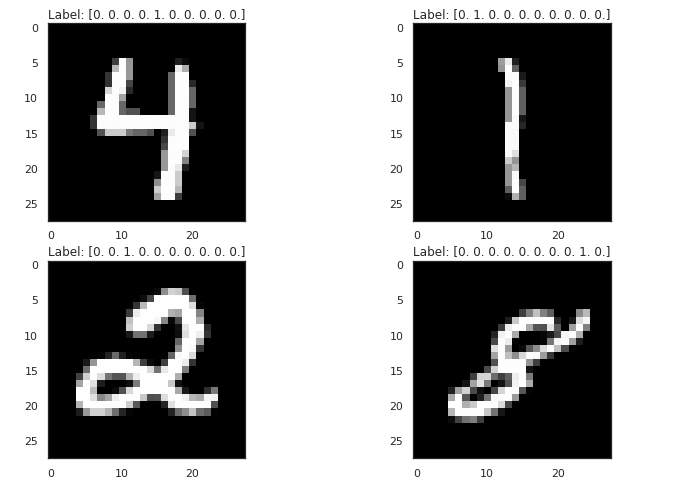
\includegraphics[width=0.8\linewidth]{img/mnist}
	\caption{}
	\label{fig:mnist}
\end{figure}

En el dataset, las imágenes están representadas como un conjunto de píxeles organizados por filas, donde cada píxel es un unsigned byte que toma un valor entre 0 y 255 (el 0 indica que ese píxel es blanco y el 255 indica que es negro). Las etiquetas de cada conjunto de datos (entrenamiento y test), por su parte, se encuentran en archivos separados y toman un valor de entre 0 y 9.

El conjunto de entrenamiento está formado por 30000 imágenes con dígitos escritos por empleados de una oficina de EEUU y 30000 imágenes 
con dígitos escritos por estudiantes de instituto. En el conjunto de test, las primeras 5000 imágenes contienen dígitos escritos por los empleados de la oficina, por lo que son más entendibles, mientras que las últimas 5000 imágenes continen dígitos escritos por los estudiantes de instituto, de manera que son más difíciles de clasificar. 

Así pues, conociendo el problema y el formato de nuestros conjuntos de datos, pasamos a estudiar distintos modelos para resolver el problema planteado y analizar los resultados que ofrecen. 

\newpage
\section{Algoritmos}

Para resolver este problema, como problema de clasificación que es, se puede usar cualquiera de los clasificadores estudiados hasta ahora en la asignatura (SVM,Knn,Random Forest, Gradient Boosting, Redes Neuronales,etc). Sin embargo, para usar estos algoritmos hay que convertir las imágenes (matriz 2D de píxeles) en vectores (matriz 1D de píxeles), de manera que se pierde información importante a cerca de la localización espacial de cada píxel, como las distancias entre píxeles, por lo que, aunque se han llegado a conseguir buenos resultados con estos algoritmos, no son los más recomendados para este problema. 

Con el objetivo de conservar la información espacial, se hace uso de un tipo especial de redes neuronales, conocidas como \textbf{Redes Neuronales Convolucionales (CNN)}. Estas redes son las que han dado los mejores resultados en la clasificación de los dígitos de este problema, consiguiendo más del 99.8\% de precisión. Por ello, vamos a centrarnos en explicar cómo funcionan y en analizar distintas arquitecturas de las mismas.

\subsection{Redes Neuronales convolucionales}


Una Red Neuronal Convolucional recibe como entrada una imagen como un conjunto de píxeles. En concreto recibe una matriz tridimensional de píxeles, donde la primera y segunda dimensión se corresponden con el alto y ancho de la imagen y la tercera dimensión es 1 si la imagen está en escala de grises o 3 si está en color. Nos centramos en el primero de los casos pues nuestras imágenes son en blanco y negro. Sobre esta matriz de entrada se aplica una operación conocida como \underline{convolución}, con el fin de detectar ciertas características en la imagen, principalmente los bordes presentes en la misma. Esta operación consiste en aplicar sistemáticamente un filtro o kernel sobre la imagen original, el cual es una matriz de pesos con la misma profundidad que la imagen de entrada y con un número de filas y columnas normalmente bastante menor que el de la matriz de entrada. Este filtro recorre la imagen de entrada realizando su producto escalar (multiplicación píxel por píxel y suma de todos los resultados) con distintas zonas de la imagen de igual tamaño que el filtro. El resultado es una matriz de menor tamaño que la original, conocida como mapa de características, donde se ven resaltadas las características de la imagen de entrada que se pretenden detectar en la misma. En las imágenes siguientes, obtenidas del vídeo \cite{2}, se ve más claramente en qué consiste esta operación:

\begin{figure}[H]
	\centering
	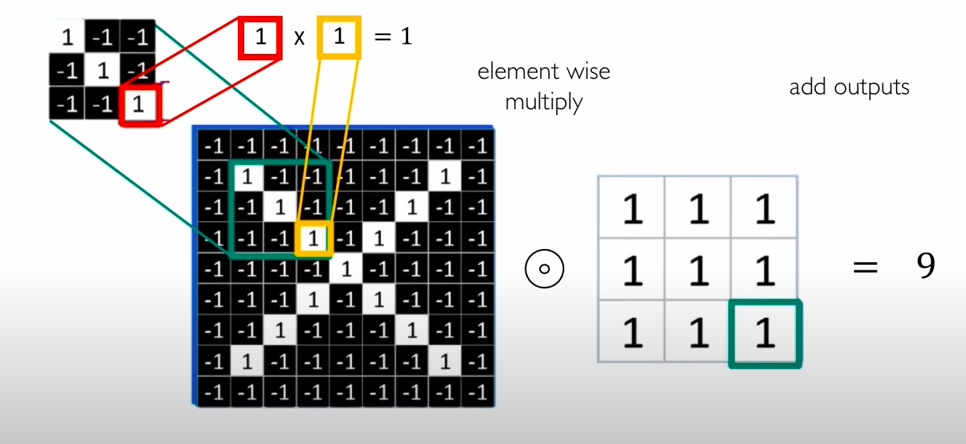
\includegraphics[width=1\linewidth]{img/conv1}
	\caption{}
	\label{fig:conv1}
\end{figure}
\begin{figure}[H]
	\centering
	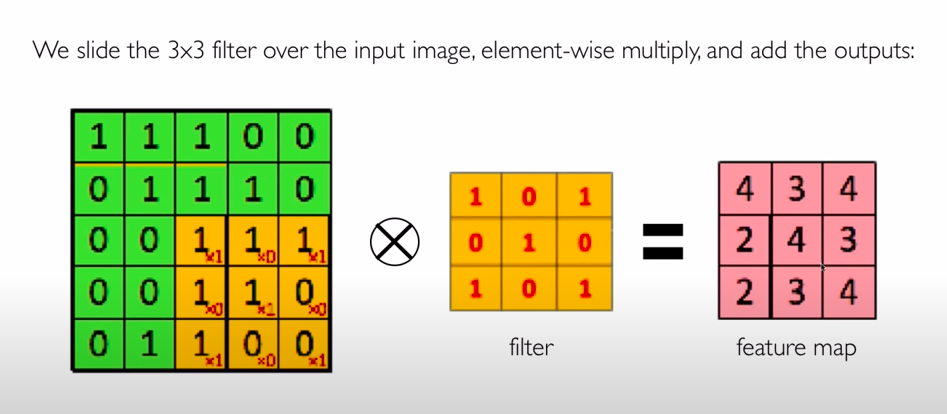
\includegraphics[width=1\linewidth]{img/conv2}
	\caption{}
	\label{fig:conv2}
\end{figure}

Se pueden aplicar varios filtros sobre la imagen de entrada para detectar diferentes características, en cuyo caso el mapa de características resultante tendrá una profundidad igual al número de filtros aplicados:

\begin{figure}[H]
	\centering
	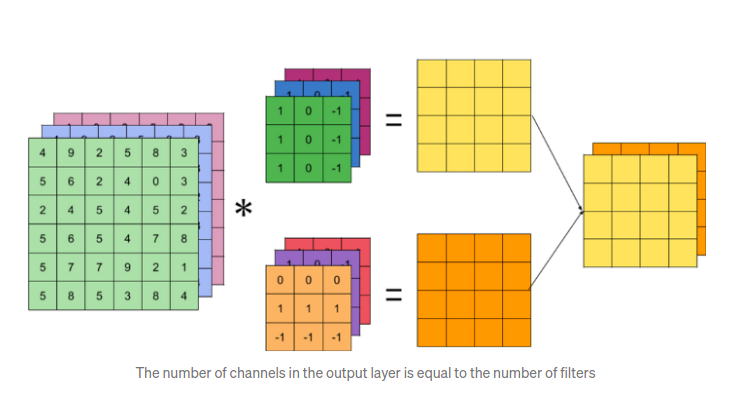
\includegraphics[width=1\linewidth]{img/conv3}
	\caption{}
	\label{fig:conv3}
\end{figure}

Los pesos de cada uno de los filtros son aprendidos por la red durante el proceso de entrenamiento. 


A veces, puesto que los píxeles en las esquinas de la imagen de entrada son considerados sólo una vez en la operación de convolución y se puede perder información contenida en los mismos, se agranda la imagen de entrada, añadiéndole bordes de ceros de manera que las esquinas de la nueva imagen no contendrán información y las esquinas de la imagen original serán recorridas más de una vez por el filtro. Esto es lo que se conoce como \textit{padding}.

\begin{figure}[H]
	\centering
	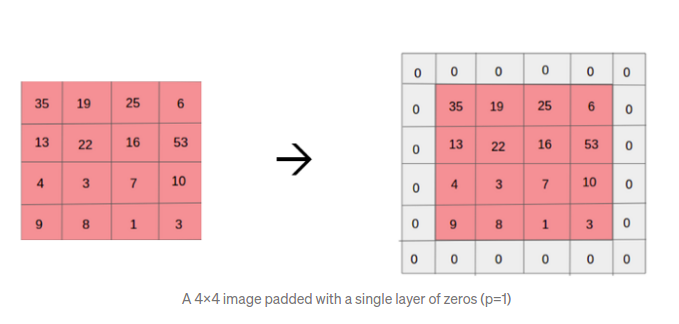
\includegraphics[width=0.8\linewidth]{img/conv4}
	\caption{}
	\label{fig:conv4}
\end{figure}

Otro concepto que se usa en el ámbito de las redes convolucionales es el \textit{stride}, que determina el número de píxeles que se mueve el filtro cada vez sobre la imagen de entrada. Así, cuanto mayor sea el stride, más pequeña será la matriz de salida, por lo que es útil si la imagen es muy grande. Si el stride es demasiado elevado puede que el filtro no recorra toda la imagen de entrada y haya píxeles cuya información se pierda. 

Después de cada operación de convolución se aplica una \underline{función de activación} a los elementos de la matriz resultante para romper la linealidad del modelo. La más frecuente es la función ReLu, que cambia los valores negativos por 0 y deja inalterados los valores positivos.

Para reducir el tamaño de los mapas de características de manera que el número de parámetros que tiene que aprender la red y el coste computacional se vea reducido, se lleva a cabo una operación llamada \underline{Pooling}. Esta operación consiste en resumir las características presentes en las distintas regiones del mapa de características generado por una capa convolucional de la red sin que se pierda información y es llevada a cabo por una capa de 'pooling' (\underline{pooling layer}).

La operación de Pooling más frecuente es el \textit{Max Pooling}, que selecciona el elemento que presenta el valor más alto de cada región del mapa de características, con lo que la salida de esta  operación será un mapa de características conteniendo las características más destacadas del mapa de entrada. 

\begin{figure}[H]
	\centering
	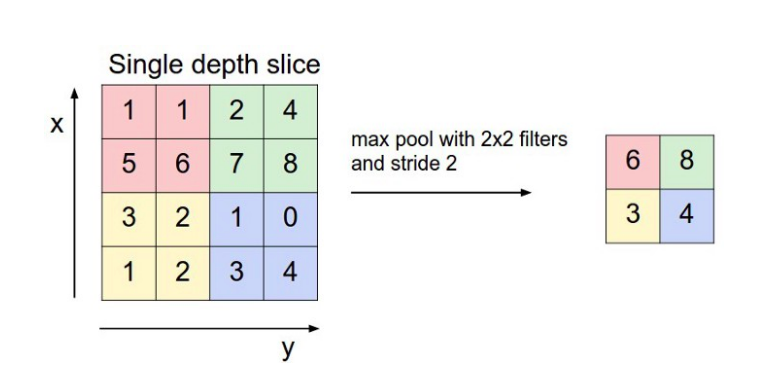
\includegraphics[width=0.8\linewidth]{img/cov5}
	\caption{}
	\label{fig:cov5}
\end{figure}


Existen otro tipo de operaciones de Pooling, como el \textit{Average Pooling}, que toma la media de los valores presentes en cada región del mapa de características de tamaño igual al del filtro considerado. 

\begin{figure}[H]
	\centering
	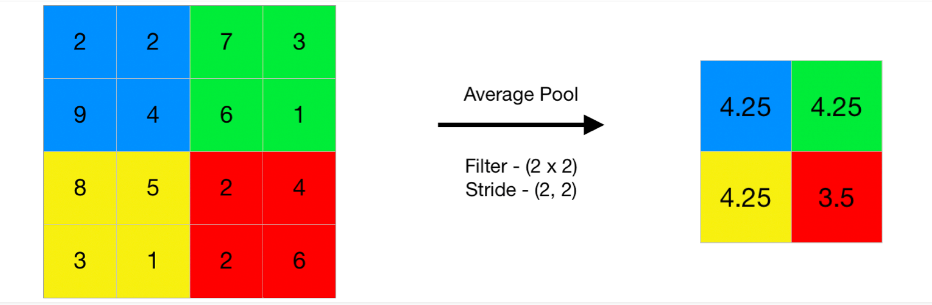
\includegraphics[width=0.8\linewidth]{img/conv9}
	\caption{}
	\label{fig:conv9}
\end{figure}


Así pues, es bastante común que en una red convolucional se use una capa de Pooling tras una capa de convolución para reducir el tamaño de la salida de esta última. 

Una vez que las capas convolucionales han extraído las características más importantes de la imagen de entrada, se convierte la salida resultante de estas en un vector unidemensional que es usado como entrada para cualquier clasificador, el cual se encargará de clasificar la imagen original en su correspondiente clase usando la información que han extraído las capas convolucionales. Lo más común es que se usen redes neuronales para realizar esta clasificación, cuyas capas se conocen como Fully-connected layers (cada nodo de la capa anterior está conecado con cada nodo de la siguiente capa), donde la última capa tiene como función de activación la función softmax, la cual determina la probabilidad de que la imagen original pertenezca a cada una de las clases consideradas en el problema. 

En resumen, la estructura de una red convolucional es generalmente la que se muestra en las siguientes figuras:
\begin{figure}[H]
	\centering
	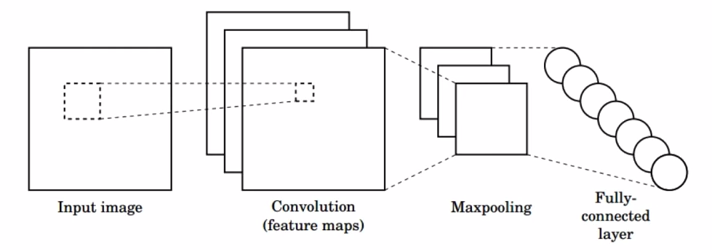
\includegraphics[width=1\linewidth]{img/con7}
	\caption{}
	\label{fig:con7}
\end{figure}
\begin{figure}[H]
	\centering
	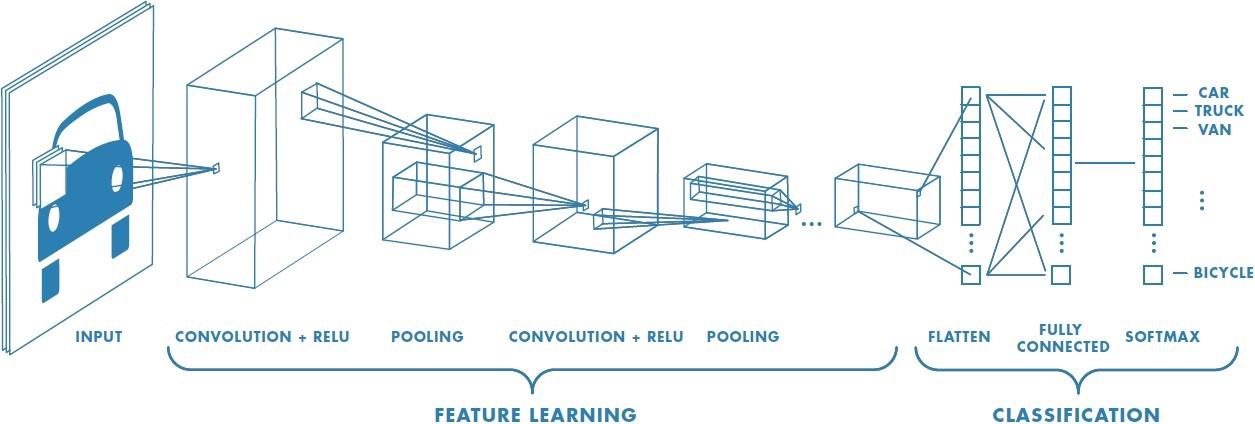
\includegraphics[width=1\linewidth]{img/conv6}
	\caption{}
	\label{fig:cov5}
\end{figure}

\subsection{Arquitectura LeNet-5}

LeNet-5 es un tipo de arquitectura de redes neuronales convolucionales bastante antigua, introducida por primera vez en el paper \cite{7} de Yann André LeCun, Leon Bottou, Yoshua Bengio, y Patrick Haffner, para resolver, de hecho, el problema que nos ocupa.

Esta arquitectura está formada por un total de 7 capas, dos capas convolucionales y otras dos capas de average pooling seguidas por tres 'fully-connected layers',  siendo una de ellas la capa de salida. 

\begin{figure}[H]
	\centering
	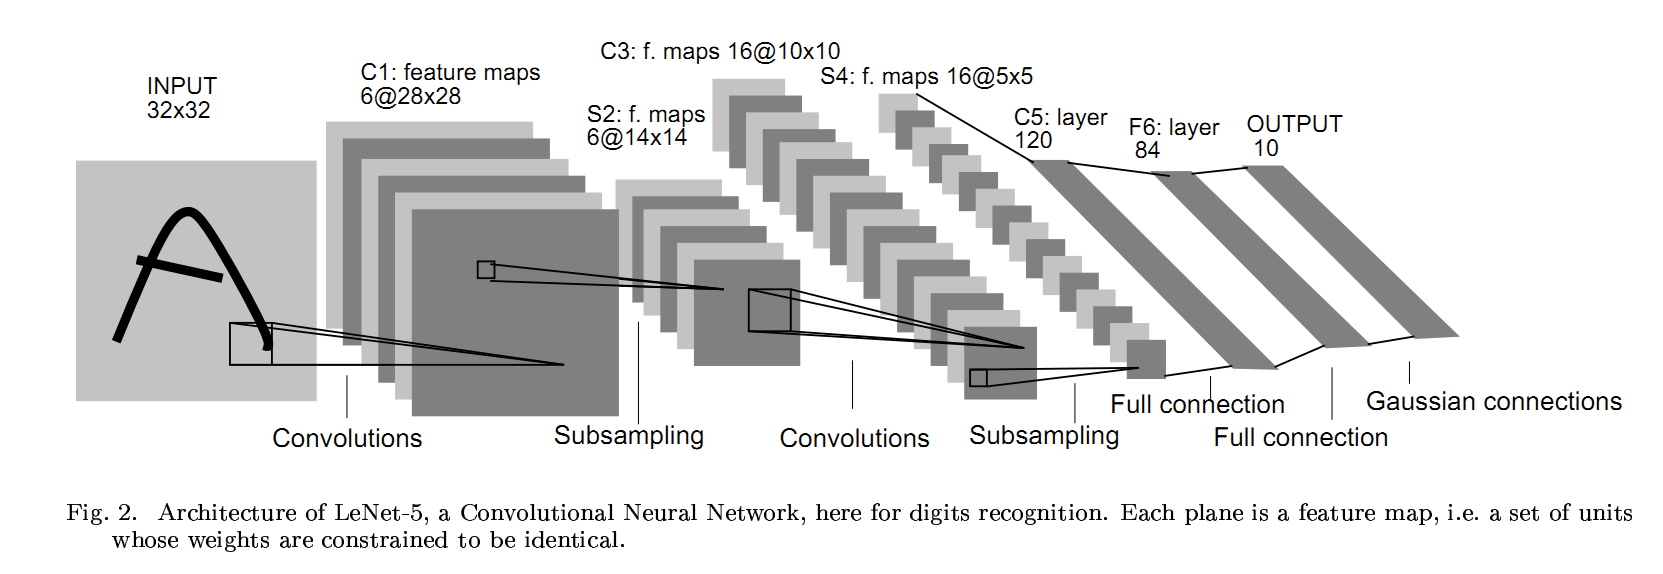
\includegraphics[width=1.1\linewidth]{img/lenet}
	\caption{}
	\label{fig:lenet}
\end{figure}

\begin{enumerate}
	\item La \underline{capa de entrada} toma una imagen de tamaño  32x32, que es pasada a la primera capa convolucional (C1). Puesto que las imágenes del dataset MNIST tienen tamaño  28x28 , es necesario aplicar padding a las mismas para obtener imágenes de  32x32 . 
	\item Sobre la imagen de entrada se aplican en \underline{la primera capa convolucional (C1)} 6 filtros de tamaño  5x5  con un stride de 1, obteniéndose 6 mapas de características como salida de tamaño  28x28 . 
	\item A C1 la sigue una \underline{capa de subsampling (S2)}, que es básicamente una capa de Pooling que reduce a la mitad el tamaño de los mapas resultantes de C1, aplicando una operación de Average Pooling con un tamaño de filtro de 2x2 y un stride de 2. Así, la salida de esta capa son 6 mapas de características con dimensiones  14x14 .
	\item A continuación viene otra \underline{capa de convolución (C3)}, formada por 16 filtros  10x10,  que se aplican sobre diferentes combinaciones de los 6 mapas de características que proporciona S2 como salida, obteniendo 16 mapas de características de tamaño  10x10 
	\item \underline{S4 es otra capa de subsampling} con exactamente la misma estructura y función que S2, de manera que como resultado de esta tenemos 16 mapas de tamaños  5x5 
	\item La capa 5 es una \underline{capa de convolución 'fully-connected' (C5)} con 150 nodos, donde cada uno de ellos está conectado con cada uno de los  5x5x16=400   elementos de los mapas de características a la salida de S2.
	\item \underline{F6} es una capa de red neuronal convencional (también 'fully-connected') constituida por 84 nodos conectados con los 120 nodos de la capa anterior. 
	\item La \underline{capa de salida} consta de 10 neuronas conectadas con las 84 de F6 que aplican la función de activación softmax y da 10 valores como salida correspondientes a las probabilidides de que la imagen de entrada original pertenezca a cada una de las clases del problema (dígitos 0 a 9).
\end{enumerate}

En la siguiente tabla podemos ver un resumen de las diferentes capas de esta arquitectura:


\begin{figure}[H]
	\centering
	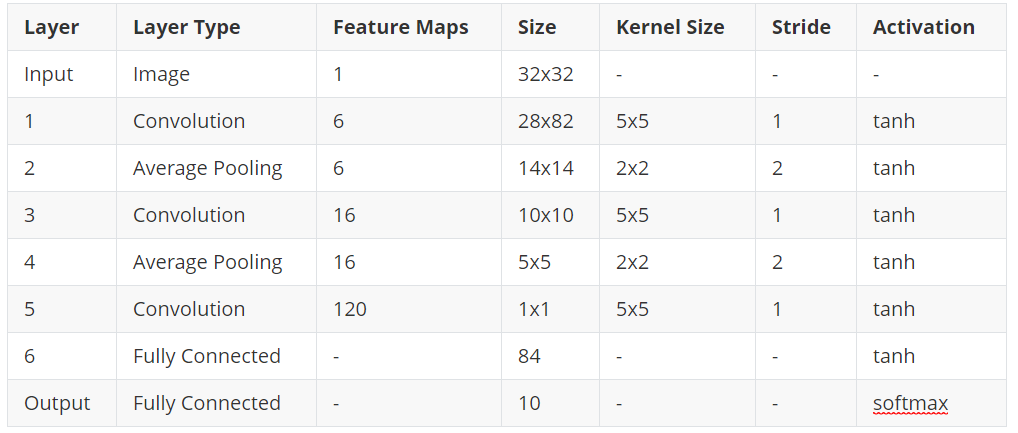
\includegraphics[width=1\linewidth]{img/lenet2}
	\caption{}
	\label{fig:lenet2}
\end{figure}

\subsection{Arquitectura VGGNet}

Esta es otro tipo de arquitectura de redes convolucionales propuesta por Karen Simonyan y Andrew Zisserman en 2014. Está diseñada para imágenes de entrada en color (RGB) y de tamaño 224x224. Cuenta con un total de 13 capas convolucionales y 3 capas fully-connected en la variante \textbf{VGG16} y 16 capas convolucionales y 3 fully-connected en la variante \textbf{VGG19}. Ambas variantes presentan además 5 capas de Max Pooling idénticas (tamaño de filtro 2x2 y stride 2) que se intercalan entre las capas convolucionales. 

Los filtros de las capas convolucionales son todos de pequeño tamaño, 3x3, pues la idea de esta arquitectura es tener redes más profundas con filtros más pequeños en lugar de filtros grandes (y por lo tanto con más parámetros) y un profundidad menor. Además, el stride es 1 para todos los filtros y en cada capa convolucional se aplica padding de manera que las salidas tengan el mismo tamaño que las entradas.

Las capas totalmente conectadas (fully-connected) constan de 4096 nodos, las dos primeras, y 1000 nodos, la tercera, para predecir las 1000 clases de las que dispone el problema para el que esta red fue diseñada (ImageNet). Así, para poder usar esta arquitectura en nuestro problema, debemos modificar ligeramente algunos aspectos de la misma y de nuestros datos, que veremos en la parte experimental.

Cabe mencionar que las estructuras de redes convolucionales que probamos en~\ref{subsection:my} se basan en este tipo de arquitectura, aunque son mucho más sencillas y menos profundas. 

La estructura detallada de ambas variantes de VGGNet se puede ver en la Figura 11, y la Figura 12 muestra la arquitectura de VGG16:

\begin{figure}[H]
	\centering
	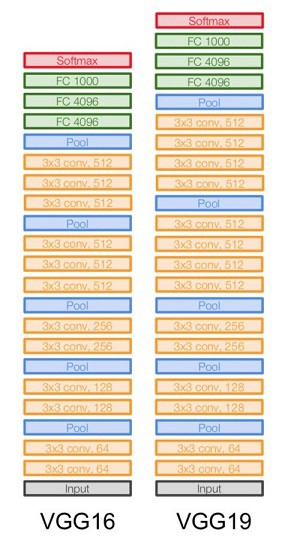
\includegraphics[width=0.6\linewidth]{img/vgg1}
	\caption{}
	\label{fig:vgg1}
\end{figure}

\begin{figure}[H]
	\centering
	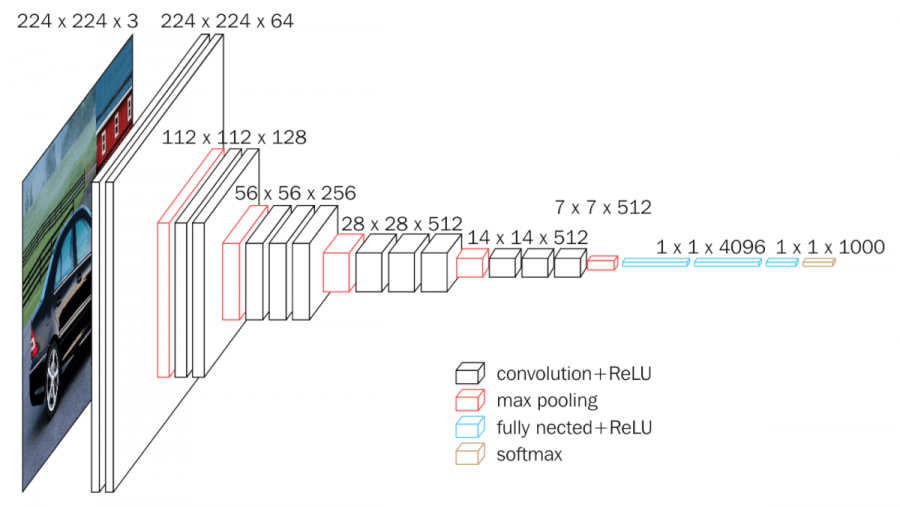
\includegraphics[width=1\linewidth]{img/vgg2}
	\caption{}
	\label{fig:vgg2}
\end{figure}

\subsection{Transfer Learning}

Transfer Learning es el proceso que consiste en tomar un modelo ya pre-entrenado sobre un conjunto de datos, es decir, los pesos (en el caso de las redes neuronales) y demás parámetros del modelo ya han sido aprendidos, y aplicar ese modelo a otro problema parecido al problema para el que fue entrenado. Normalmente se vuelve a entrenar el modelo sobre el conjunto de datos del nuevo problema considerado para que los parámetros del modelo se ajusten mejor a los nuevos datos, pero partiendo de los parámetros que ya tenía aprendidos, de forma que el aprendizaje será más rápido y se necesitarán menos datos para un correcto aprendizaje. Este proceso de volver a entrenar el modelo sobre el nuevo conjunto de datos es lo que se conoce como \textit{fine-tuning}. 


 Para nuestro caso, consideramos redes convolucionales pre-entrenadas. Hay muchas formas de usar estas redes pre-entrenadas:
\begin{itemize}
	\item Lo más fácil y común es eliminar la última capa de la red ya entrenada (que será la que se encarga de hacer la clasificación en el problema para el que fue entrenada) y añadirle otra capa sin entrenar, que es a continuación entrenada sobre el nuevo conjunto de datos manteniendo fijos los parámetros del resto de la red. La parte fija actuaría en este caso como 'extractor de características' y la última capa sería la encargada de realizar la clasificación. Este método se usa si los datos del problema para el que queremos usar la red son bastante parecidos a los datos sobre los que la red fue entrenada originalmente.  
	\begin{figure}[H]
		\centering
		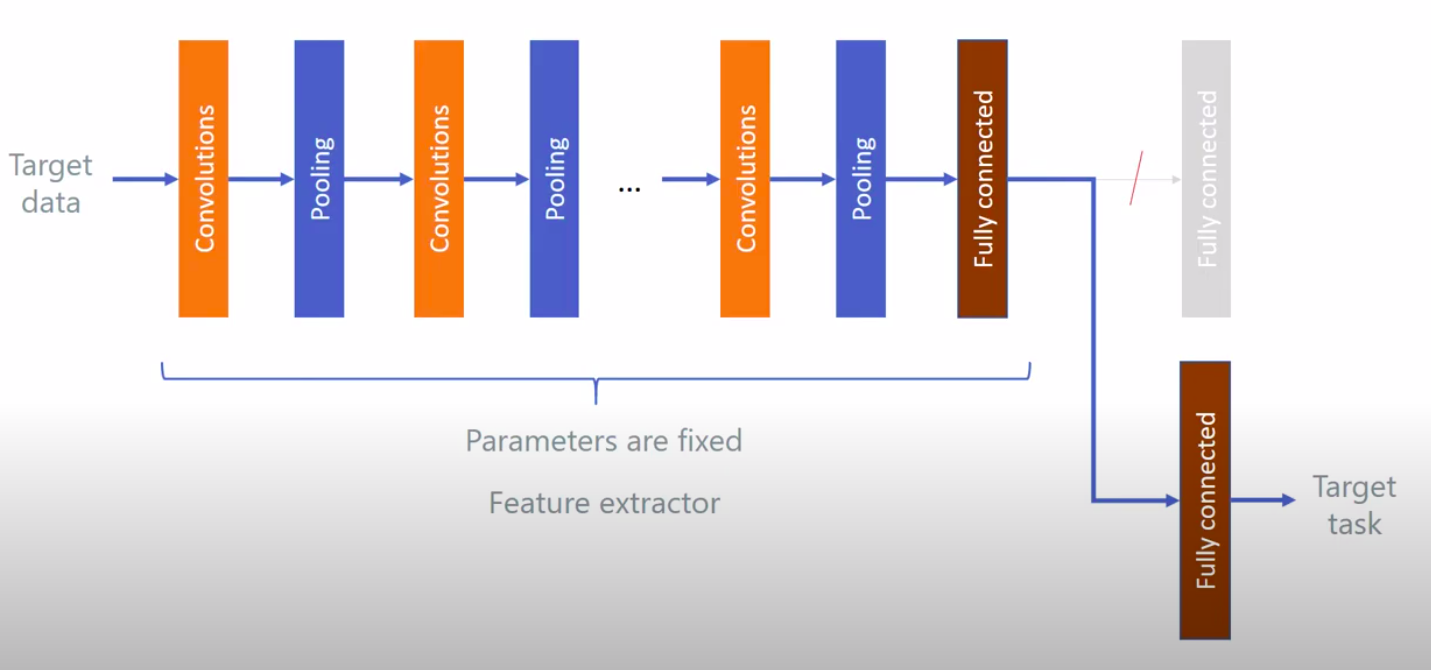
\includegraphics[width=0.9\linewidth]{img/tl1}
		\caption{}
		\label{fig:tl1}
	\end{figure}
	
	\item Si nuestro dataset dispone de una cantidad considerable de datos, podemos hacer un fine-tuning de la red completa (una vez ya entrenada la última capa habiendo congelado las primeras capas) partiendo de los parámetros ya aprendidos. Si, por el contrario, nuestro data set es pequeño, un fine-tuning puede llevar a un sobreajuste de la red al conjunto de entrenamiento.
	
	\item Otra opción es considerar únicamente las n primeras capas de la red pre-entrenada, fijar sus parámetros y entrenar desde cero el resto de las capas sobre el nuevo conjunto de datos. Puesto que las primeras capas de una red convolucional (o red neuronal convencional) se encargan de extraer las características generales de los datos de entrada (como los bordes, curvas, esquinas, etc), si nuestro problema no es muy parecido al problema para el que la red fue entrenada, podemos considerar sólo las capas iniciales, que extraerán las carácterísticas generales que son comunes a los dos problemas. La últimas capas de la red son las que aprenden las características más específicas del problema, por lo que, cuanto menos parecido sea nuestro problema, entrenaremos desde cero un mayor número de las últimas capas, es decir, menos capas de la red pre-entrenada consideraremos fijas. 
	\begin{figure}[H]
		\centering
		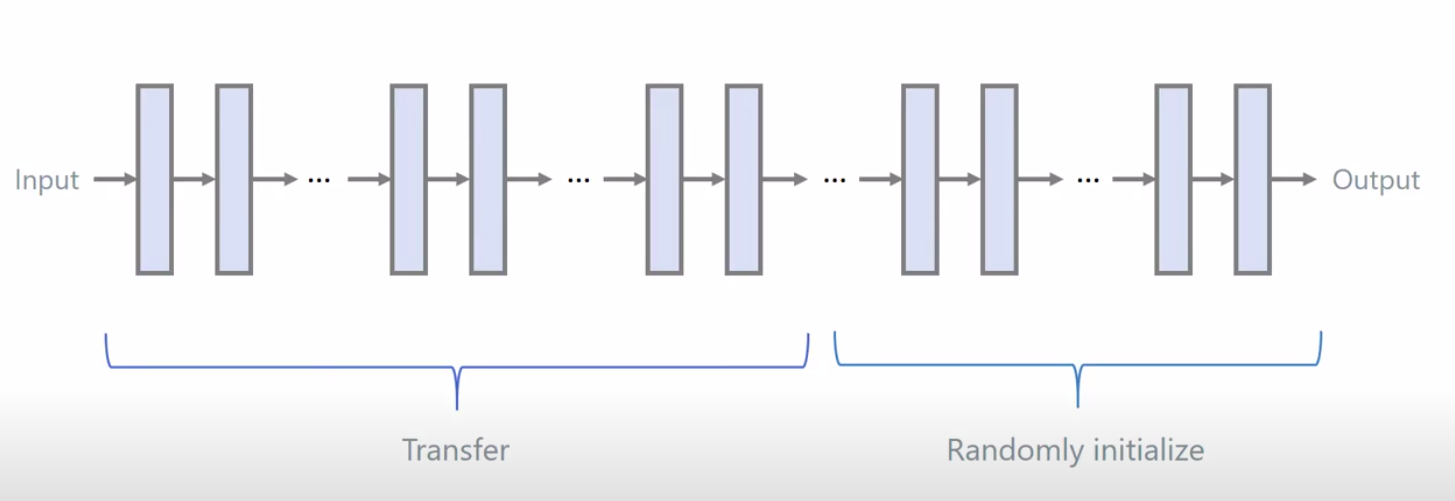
\includegraphics[width=0.9\linewidth]{img/tf2}
		\caption{}
		\label{fig:tf2}
	\end{figure}

\end{itemize}
 
 Este técnica permite que el entrenamiento de la red se centre en las partes de la misma que son más importantes para nuestro problema (normalmente las últimas capas) porque se encargan de extraer características específicas del mismo, 'olvidándose' del resto de capas, que extraen características comunes a muchos problemas y que ya han sido entrenadas, haciendo que el aprendizaje sea más rápido. 

\newpage
\section{Estudio experimental}
\subsection{LeNet-5}
Para probar esta arquitectura he implementado un código (\mintinline{python}{lenet.ipynb}) usando la biblioteca de python \mintinline{python}{Keras} y basado en el código que se puede encontrar en \cite{10}. 
\subsubsection{Lectura de los datos y preprocesamiento}
En primer lugar, hay que descargarse los conjuntos de datos de su página oficial \cite{11} y cargarlos como aparece en \cite{12}. Una vez cargados, los convertimos en arrays y le damos el tamaño apropiado a cada uno. 
\begin{minted}{python}
x_train, y_train = mndata.load_training()
x_test, y_test = mndata.load_testing()

x_train = np.asarray(x_train)
y_train = np.asarray(y_train)
x_test = np.asarray(x_test)
y_test = np.asarray(y_test)

x_train = x_train.reshape((len(x_train),28,28))
x_test = x_test.reshape((len(x_test),28,28))
\end{minted}

Normalizamos ahora las imágenes en escala de grises, cuyos píxeles presentan valores entre 0 y 255, a valores entre 0 y 1, dividiendo el valor de cada uno de los píxeles entre 255. Además, le damos 4 dimensiones a los conjuntos de datos:
\begin{minted}{python}
#normalization
x_train = x_train / 255.0
x_test = x_test / 255.0

#reshape
x_train = x_train.reshape(-1, 28,28,1)
x_test = x_test.reshape(-1, 28,28,1)
\end{minted}

Para esta arquitectura es necesario que las imágenes tengan tamaño 32x32, por lo que le añadimos a todas, tanto del conjunto de entrenamiento como de test, un padding de 2:
\begin{minted}{python}
# Padding the input to make it 32x32. Specification of LeNET
x_train = np.pad(x_train, [(0, 0), (2, 2), (2, 2), (0, 0)], "constant") 
x_test = np.pad(x_test, [(0, 0), (2, 2), (2, 2), (0, 0)], "constant") 
\end{minted}

Por otra parte, convertimos los valores numéricos de las etiquetas (de 0 a 9) a un 'one-hot encoded vector' cada uno, para que dichas etiquetas sean tratadas como categorías con igual importancia en lugar de números con orden:
\begin{minted}{python}
#label encoding
y_train = to_categorical(y_train, num_classes=10)
y_test = to_categorical(y_test, num_classes=10)
\end{minted}

Finalmente, dividimos el conjunto de datos de entrenamiento original en dos subconjuntos, uno de entrenamiento y otro de validación, de manera que los conjuntos de datos resultantes tendrán los siguientes tamaños:

\begin{minted}{python}
	X_train shape:  (54000, 32, 32, 1)
	X_val shape:  (6000, 32, 32, 1)
	y_train shape:  (54000, 10)
	y_val shape:  (6000, 10)
\end{minted}

\subsubsection{Construcción del modelo}
Para construir la arquitectura LeNet, usamos la clase \mintinline{python}{Sequential} de Keras, que apila el conjunto de capas que le indiquemos una detrás de otra y las va ejecutando de manera secuencial. Usaremos las capas \mintinline{python}{Conv2D()}, correspondiente a una capa convolucional, \mintinline{python}{AveragePooling2D()}, que realiza la operación de average pooling, \mintinline{python}{Flatten()}, que convierte una matriz 2D de entrada en una matriz 1D de salida y \mintinline{python}{Dense()}, correspondiente a una capa de red neuronal convencional fully-connected. Teniendo en cuenta las características de cada una de las capas de la arquitectura LeNet que aparecen en la Figura 10, construimos el modelo como sigue:
\begin{minted}{python}
model = Sequential()

model.add(Conv2D(filters=6, kernel_size = (5,5), padding = 'valid', activation= 'tanh', 
input_shape = (32,32,1),strides=(1,1)))
model.add(AveragePooling2D(pool_size = (2,2),strides=(2,2)))

model.add(Conv2D(filters=16, kernel_size = (5,5), padding = 'valid', activation= 'tanh',
strides=(1,1)))
model.add(AveragePooling2D(pool_size = (2,2),strides=(2,2)))

model.add(Flatten())
model.add(Dense(120, activation = 'tanh'))
model.add(Dense(84, activation = 'tanh'))
model.add(Dense(10, activation = 'softmax'))
\end{minted}
donde \mintinline{python}{padding='valid'} indica que no se aplique padding. El resumen del modelo construido es entonces el siguiente:
\begin{figure}[H]
	\centering
	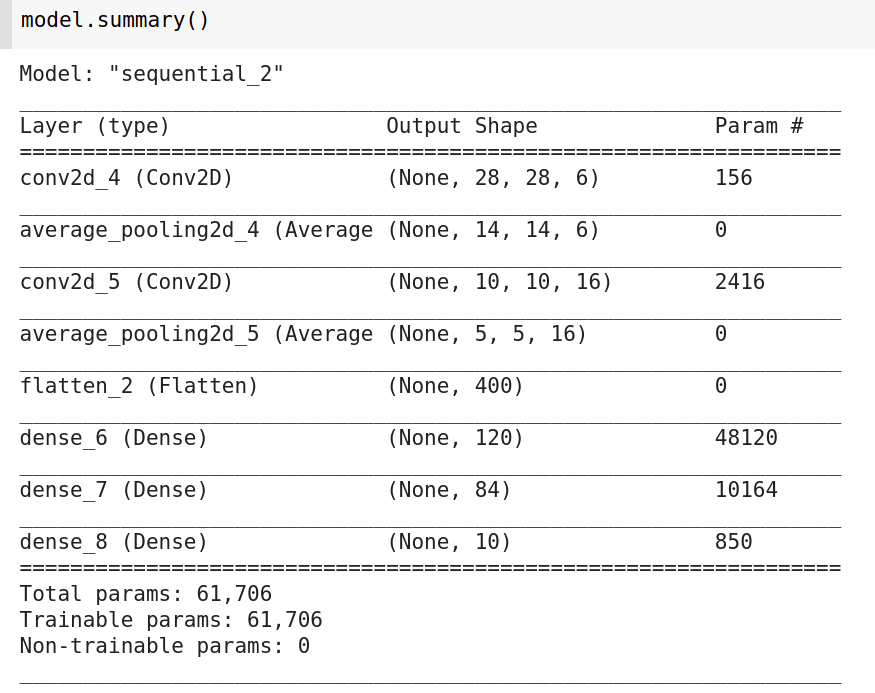
\includegraphics[width=0.8\linewidth]{img/lenet3}
	\caption{}
	\label{fig:lenet3}
\end{figure}
 A continuación configuramos el modelo para el entrenamiento, indicando que vamos a usar el algoritmo 'Adam' como optimizador, 'cross-entropy' como función de pérdida (esta mide las diferencias entre las categorías predichas y las reales) y accuracy como métrica para medir la calidad del modelo. Además, consideraremos un tamaño de batch de 86 y 50 épocas (epochs), que es el número de veces que el modelo va a pasar sobre el conjunto de entrenamiento completo durante el proceso de entrenamiento. 
\begin{minted}{python}
model.compile(optimizer = 'adam', loss = 'categorical_crossentropy',
metrics = ['accuracy'])

epochs = 50 
batch_size = 86
\end{minted}
Finalmente, entrenamos el modelo construido
\begin{minted}{python}
# Fit the model
history = model.fit(x_train,y_train, batch_size=batch_size,
epochs = epochs, validation_data = (x_val,y_val),
verbose = 2, steps_per_epoch=x_train.shape[0] // batch_size)
\end{minted}
\subsubsection{Resultados}

Usamos ahora el modelo entrenado para predecir las clases del conjunto de test y visualizamos la matriz de confusión:
\begin{figure}[H]
	\centering
	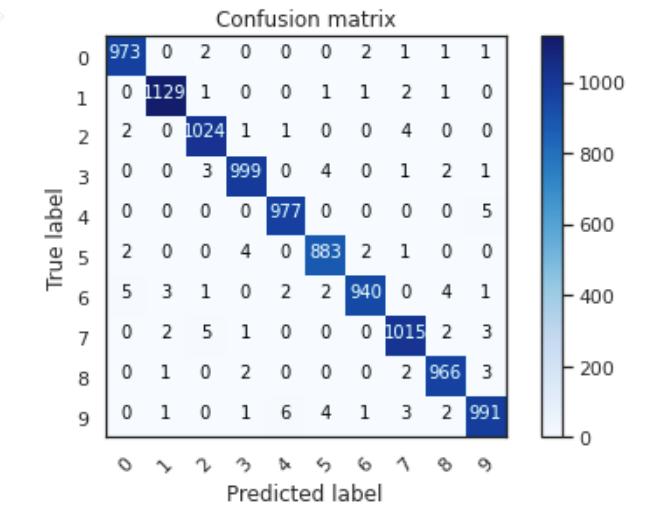
\includegraphics[width=0.8\linewidth]{img/confs1}
	\caption{}
	\label{fig:confs1}
\end{figure}

Si evaluamos el modelo sobre el conjunto de test, obtenemos la siguiente precisión: \mint{python}{Test Accuracy:  0.9897}

Por lo tanto, aunque LeNet es una arquitectura de redes convolucionales muy sencilla, presenta unos resultados muy buenos, alcanzando casi el 99\% de precisión en la clasificación y sólo un número muy pequeño de ejemplos son clasificados incorrectamente.
\subsection{Otras estructuras de CNNs sencillas}
\label{subsection:my}
Buscando códigos que participaron en la competición de Kaggle para resolver el problema del reconocimiento de dígitos \cite{13}, encontré el código de \cite{14}, que alcanzaba el 99.8\% de precisión en dicha competición, por lo que decidí probarlo sobre todo el conjunto original de MNIST e intentar entender la estructura de la red convolucional construida. En este código se presentan dos tipos diferentes de arquitecturas que a continuación detallamos.

\subsubsection{Doble capa convolucional}
\textbf{Lectura de datos y preprocesamiento}

Se siguen exactamente los mismos pasos explicados en la arquitectura anterior, salvo que en este caso no es necesario hacer padding a las imágenes originales, pues la primera capa de la red recibe las imágenes con tamaño 28x28 directamente.

\textbf{Construcción del modelo}

El modelo construido es el siguiente:
\begin{minted}{python}
model = Sequential()

model.add(Conv2D(filters=32, kernel_size = (5,5), padding = 'Same', activation= 'relu',
input_shape = (28,28,1)))
model.add(Conv2D(filters=32, kernel_size = (5,5), padding = 'Same', activation= 'relu'))
model.add(MaxPool2D(pool_size = (2,2)))
model.add(Dropout(0.25))

model.add(Conv2D(filters=64, kernel_size = (3,3), padding = 'Same', activation= 'relu'))
model.add(Conv2D(filters=64, kernel_size = (3,3), padding = 'Same', activation= 'relu'))
model.add(MaxPool2D(pool_size = (2,2), strides = (2,2)))
model.add(Dropout(0.25))

model.add(Flatten())
model.add(Dense(256, activation = 'relu'))
model.add(Dropout(0.5))
model.add(Dense(10, activation = 'softmax'))
\end{minted}

\begin{figure}[H]
	\centering
	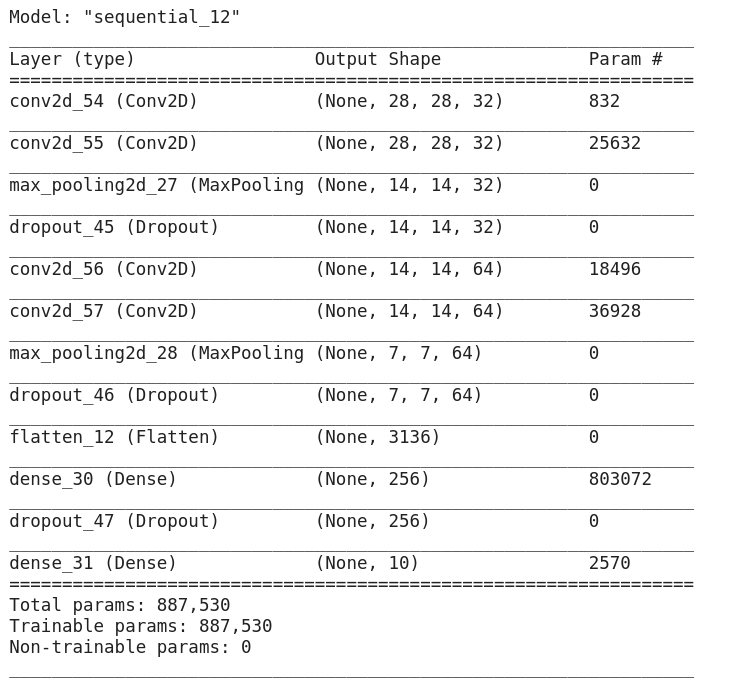
\includegraphics[width=0.8\linewidth]{img/cnn1}
	\caption{}
	\label{fig:cnn1}
\end{figure}

Tenemos en primer lugar dos capas convolucionales con 32 filtros cada una de tamaño 5x5 que reciben como entrada una imagen de tamaño 28x28 y producen como salida 32 mapas de características del mismo tamaño, pues se aplica un padding al resultado para que la salida sea del mismo tamaño que la entrada (\mintinline{python}{padding='same'}). A continuación viene una capa de Pooling, que realiza la operación de Max Pooling sobre los mapas de características resultantes de las dos primeras capas convolucionales, con un tamaño de filtro de 2x2 y un stride también de 2, de manera que el resultado son 32 mapas de características con un tamaño igual a la mitad del tamaño de entrada (14x14). 

Para reducir el overfitting, se introduce una capa \mintinline{python}{Dropout(0.25)}, que pone a 0 el 25\% de los elementos de entrada elegidos de manera aleatoria y el resto son aumentados en $ 1/0.75 $, de manera que la suma de todos los elementos de la entrada permanece invariante. 

Después encontramos otra pareja de capas convolucionales, esta vez con 64 filtros de tamaño 3x3, que dan 64 mapas de características de tamaño 14x14 (igual que la entrada) debido a la operación de padding. Tras estas dos capas, volvemos a tener una capa de Max Pooling con la misma estructura que la primera que se introdujo, y produce como salida 64 mapas de tamaño 7x7. A esta la sigue otra capa de drop out para evitar el overfitting. 

Tras estas dos parejas de capas convolucionales, vienen las capas fully-connected, las cuales reciben como entrada un vector, por lo que primero se usa una capa \mintinline{python}{Flatten()} para convertir los mapas de características en un vector de tamaño $7*7*64=3136$.  La primera de estas capas consta de 256 nodos y va seguida por una capa de drop out con una frecuencia de 50\% de anulación de elementos. La siguiente capa es la de salida, con 10 nodos correspondientes a cada una de las 10 clases de nuestro problema. 

Para el entrenamiento se usa como optimizador el algoritmo de \textit{'Root Mean Square Propagation (RMSProp)'} y como función de pérdida 'cross-entropy'. Además, durante el entrenamiento se usa la clase \mintinline{python}{ReduceLROnPlateau}, que se encarga de reducir el \textit{learning rate} en un factor de $ 0.5$ en este caso si no hay disminución en la función de pérdida tras 3 epochs (\mintinline{python}{patience=3}):
\begin{minted}{python}
optimizer = RMSprop(lr = 0.001, rho = 0.9, epsilon=1e-08, decay =0.0)

model.compile(optimizer = optimizer, loss = 'categorical_crossentropy', 
metrics = ['accuracy'])

learning_rate_reduction = ReduceLROnPlateau(monitor='val_loss', 
	patience=3, 
	verbose=1, 
	factor=0.5, 
	min_lr=0.00001)
\end{minted}

Consideramos, como para el entrenamiento de la red LeNet, un batch size de 86 y un total de 50 épocas. 

En este caso además se lleva a cabo un aumento del conjunto de datos de entrenamiento, lo que se conoce como \textit{data augmentation}, usando \mintinline{python}{ImageDataGenerator}. Este proceso consiste en crear nuevas imágenes modificando ligeramente las imágenes originales del conjunto de datos de entrenamiento, como por ejemplo haciendo zoom en ellas, rotándolas un cierto ángulo, desplazando todos los píxeles horizontal o verticalmente, etc. Estas técnicas mencionadas son las que  aquí se aplican sobre nuestro conjunto de datos para aumentarlo. De este modo la red dispone de muchas más imágenes con las que entrenar ligeramente diferentes entre sí, lo que ayuda a que el resultado tras el entrenamiento sea mejor. 
\begin{minted}{python}
#Data Augmentation
datagen = ImageDataGenerator(
# set input mean to 0 over the dataset
featurewise_center=False, 
# set each sample mean to 0
samplewise_center=False, 
# divide inputs by std of the dataset
featurewise_std_normalization=False,  
# divide each input by its std
samplewise_std_normalization=False,  
# apply ZCA whitening
zca_whitening=False,  
# randomly rotate images in the range (degrees, 0 to 180)
rotation_range=10,  
# Randomly zoom image 
zoom_range = 0.1,
# randomly shift images horizontally (fraction of total width)
width_shift_range=0.1, 
# randomly shift images vertically (fraction of total height)
height_shift_range=0.1,  
# randomly flip images
horizontal_flip=False, 
# randomly flip images
vertical_flip=False) 


datagen.fit(x_train)
\end{minted}

Pasamos ya a entrenar el modelo construido y configurado sobre el conjunto de entrenamiento aumentado que genera el método \mintinline{python}{.flow()}:
\begin{minted}{python}
# Fit the model
history = model.fit(datagen.flow(x_train,y_train, batch_size=batch_size),
	epochs = epochs, validation_data = (x_val,y_val),
	verbose = 2, steps_per_epoch=x_train.shape[0] // batch_size, 
	callbacks=[learning_rate_reduction])
\end{minted}
\textbf{Resultados}

Tras entrenar el modelo, predecimos con él las etiquetas del conjunto de test y mostramos la matriz de confusión con las clasificaciones realizadas por el mismo:
\begin{figure}[H]
	\centering
	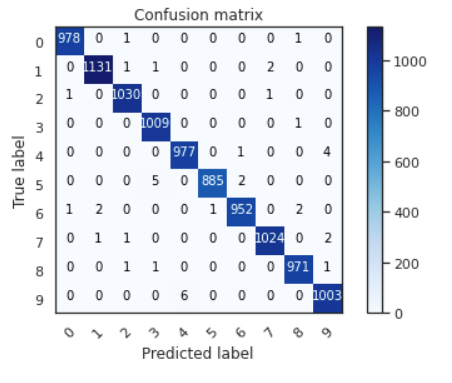
\includegraphics[width=0.7\linewidth]{img/cnn2}
	\caption{}
	\label{fig:cnn2}
\end{figure}


La precisión del modelo sobre el conjunto de test ha sido:
\mint{python}{Test Accuracy:  0.995999}

Así pues, los resultados obtenidos con este nuevo modelo superan a los que presentaba la arquitectura LeNet. Notamos, mirando las matrices de confusión de ambos modelos, que el número de ejemplos mal clasificados es bastante inferior con el nuevo modelo que con LeNet. 

Es curioso que la mayor parte de los errores se comenten al confundir el 4 con el 9. Incluso las personas no somos capaces muchas veces de distinguir estos dos números manuscritos con diferentes tipos de caligrafías, por lo que es lógico que una red neuronal también cometa este tipo de error. 

\subsubsection{Triple capa convolucional}
\textbf{Lectura de los datos y preprocesamiento}

El proceso a seguir es el mismo que en el modelo anterior.

\textbf{Construcción del modelo}

En este caso, consideramos el siguiente modelo:
\begin{minted}{python}
def get_newtriplecnn():
	return Sequential([
		Conv2D(32, kernel_size=(3, 3), activation='relu', padding='same',
		input_shape = (28,28,1)),
		Conv2D(32, kernel_size=(3, 3), activation='relu', padding='same'),
		BatchNormalization(),
		MaxPool2D(pool_size=(2, 2)),
		Dropout(0.25),
		
		Conv2D(64, kernel_size=(3, 3), activation='relu', padding='same'),
		Conv2D(64, kernel_size=(3, 3), activation='relu', padding='same' ),
		BatchNormalization(),
		MaxPool2D(pool_size=(2, 2)),
		Dropout(0.25),
		
		Conv2D(128, kernel_size=(3, 3), activation='relu', padding='same' ),
		Conv2D(128, kernel_size=(3, 3), activation='relu', padding='same' ),
		BatchNormalization(),
		MaxPool2D(pool_size=(2, 2)),
		Dropout(0.25),
		
		
		Flatten(),
		
		Dense(512, activation='relu'),
		BatchNormalization(),
		Dropout(0.5),
		
		Dense(256, activation='relu'),
		BatchNormalization(),
		Dropout(0.4),
		
		
		Dense(64, activation='relu'),
		BatchNormalization(),
		Dropout(0.3),
		
		Dense(10, activation = "softmax")

])
\end{minted}

que es bastante parecido al anterior, salvo que ahora tenemos 3 parejas de capas convolucionales, mientras que antes teníamos dos, y los filtros en todas ellas tienen un tamaño de 3x3. La primera pareja de capas convolucionales consta de 32 filtros, la segunda de 64 y la tercera de 128. 

Cada pareja va seguida ahora de una capa \mintinline{python}{BatchNormalization()}, que transforma los datos de entrada de manera que los datos de salida tienen media 0 y varianza 1, es decir, se encarga de transformar la distribución de los datos en una distribución normal (0,1). Esto hace que la red sea más estable durante el entrenamiento y se puedan usar valores de learning rate más altos, lo que acelera el proceso de aprendizaje. 

Tras la normalización de los datos, nos encontramos con capas de Max Pooling, de filtro 2x2 y stride 2 en cada caso, que reducen a la mitad el tamaño de los mapas de características resultantes de las capas convolucionales, los cuales tienen el mismo tamaño que los datos que le entran a la capa convolucional, gracias al padding. Tenemos también capas de Drop Out para evitar el overfitting. 

La parte final de la estructura cuenta con 4 capas de redes neuronales fully-connected (la primera con 512 nodos, la segunda con 256, la tercera con 64 y la última, que es la capa de salida, con 10 nodos), todas (menos la última) seguidas por una capa de Batch Normalización y otra de Dropout.
\begin{figure}[H]
	\centering
	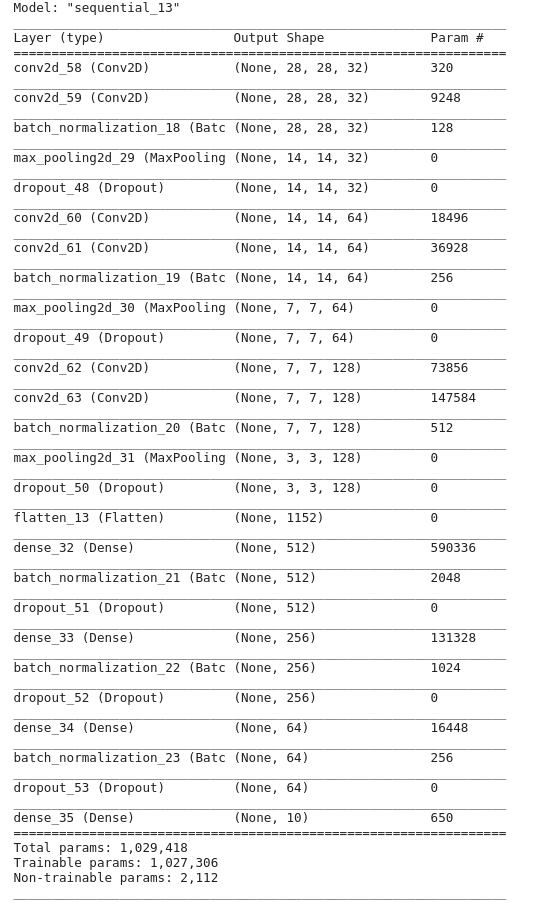
\includegraphics[width=0.8\linewidth]{img/cnn3}
	\caption{}
	\label{fig:cnn3}
\end{figure}

En este caso usamos como optimizador el algoritmo de Adam, cross-entropy como función de pérdida, accuracy como medida de la calidad del modelo y, además de hacer uso de \mintinline{python}{ReduceLROnPlateau}, como en el modelo anterior (con la diferencia de que ahora consideramos como factor de reducción del LR un 0.1), incluimos también Early Stopping, de manera que si tras 6 épocas no ha diminuido la función de pérdida, termina el entrenamiento
\begin{minted}{python}
callbacks1 = [ 
	EarlyStopping(monitor = 'loss', patience = 6), 
	ReduceLROnPlateau(monitor = 'loss', patience = 3), 
	# saving the best model
	ModelCheckpoint('model.best.hdf5', save_best_only=True) 
]
\end{minted}

Con un tamaño de batch de 86 y número de épocas de 50, procedemos a entrenar el modelo, de nuevo sobre el conjunto de entrenamiento aumentado haciendo uso de la clase \mintinline{python}{ImageDataGenerator} como comentamos en el modelo anterior
\begin{minted}{python}
history = model.fit(datagen.flow(x_train,y_train, batch_size=batch_size), epochs = 50, 
	steps_per_epoch = x_train.shape[0] // batch_size,
	validation_data = (x_val, y_val),
	callbacks = callbacks1)
\end{minted}
\textbf{Resultados}

La matriz de confusión obtenida para este modelo aplicado sobre el conjunto de test ha sido la siguiente
\begin{figure}[H]
	\centering
	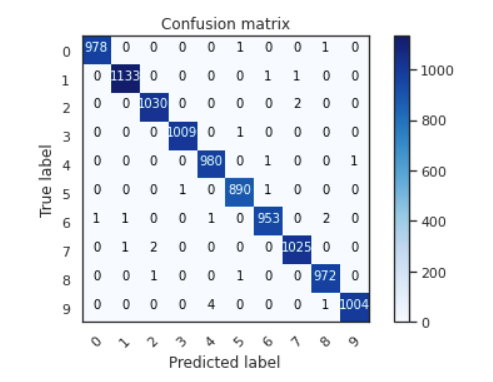
\includegraphics[width=0.8\linewidth]{img/cnn4}
	\caption{}
	\label{fig:cnn4}
\end{figure}


Y la precisión: \mint{python}{Test Accuracy:  0.9973999}

Podemos ver que las predicciones son mejores con este modelo que con los dos anteriores. Al incluir más capas convolucionales y más capas fully-connected al final, el aprendizaje ha mejorado. Teóricamente, cuanto mayor sea la profundidad de la red, mejor será la clasificación realizada por el modelo (sin tener en cuenta el overfitting que se puede producir si la red es muy profunda). Por eso, al tener ahora una red algo más profunda que la anterior, los resultados son mejores. 

\subsection{VGG16}

Para probar este tipo de arquitectura vamos a hacer uso de las redes pre-entrenadas de \mintinline{python}{Keras}, las cuales están entrenadas sobre el conjunto de datos de \textbf{ImageNet}. Puesto que las características de este conjunto de datos difieren de las de nuesto problema, vamos a tener que realizar algunas modificaciones en nuestro conjunto de datos para poder usar estas redes. Además, puesto que en ImageNet se busca clasificar las imágenes en 1000 categorías y en nuestro problema sólo queremos 10 categorías, hay que cambiar la última capa de la arquitectura VGGNet, que tiene 1000 nodos, por una capa con 10 nodos. 

Fijaremos las primeras capas de la arquitectura eliminando las capas fully-connected del final (pues estas son más específicas de ImageNet) y reemplazándolas por otras capas totalmente conectadas con un menor número de nodos y una capa de salida con 10 nodos. A continuación, entrenaremos estas últimas capas dejando fijos los parámetros de las primeras capas para finalmente hacer un fine-tuning de toda la red, de forma que se adapte mejor a nuestro problema. 

\subsubsection{Sin Data Augmentation}
\textbf{Lectura de datos y preprocesamiento}

Para leer y cargar los conjuntos de datos seguimos los mismos pasos que en los casos anteriores. El preprocesamiento es también bastante parecido salvo porque, puesto que el tamaño mínimo de imágenes de entrada que aceptan las redes VGG pre-entrenadas de Keras es 32x32 y nuestras imágenes tienen tamaño 28x28, tenemos que hacer padding a todas las imágenes, como hicimos para usar la arquitectura LeNet, para conseguir tamaño 32x32. Además, como las redes VGG esperan imágenes RGB de entrada (3 canales o profundidad 3) y las nuestras están en escala de grises (1 canal o profundidad 1), debemos copiarlas en tres canales para que sean del formato esperado por la red:
\begin{minted}{python}
	#Convert the data into 3 dimensions
	train=x_train.copy()
	test=x_test.copy()
	
	train=train.reshape(-1,32,32)
	test=test.reshape(-1,32,32)
	
	train=np.stack([train,train,train],axis=-1)
	test=np.stack([test,test,test],axis=-1)	
\end{minted}
De esta forma, los tamaños de los nuevos conjuntos serán:
\begin{minted}{python}
	x_train shape:  (60000, 32, 32, 3)
	x_test shape:  (10000, 32, 32, 3)
\end{minted}

El resto del preprocesamiento es igual que en los modelos estudiados antes. 

\textbf{Construcción del modelo}

Para construir el modelo implementamos lo siguiente:
\begin{minted}{python}
def nuevoVGG16():
	model = Sequential()
	
	model.add(VGG16(weights='imagenet', include_top=False, input_shape = (32,32,3)))
	
	
	model.add(Flatten())
	model.add(Dense(512, activation = 'relu'))
	model.add(Dropout(0.5))
	model.add(Dense(10, activation = 'softmax'))
	
	return model
\end{minted}

donde \mintinline{python}{VGG16()} instancia una red con arquitectura VGG16. A esta función le indicamos que el tamaño de las imágenes de entrada será de (32,32,3), que queremos usarla con los pesos ya aprendidos al haberla entrenado previamente sobre el conjunto de datos de ImageNet (\mintinline{python}{weights='imagenet'}) y que no se incluyan las capas fully-connected que presenta el modelo al final (\mintinline{python}{include_top=False}), pues ya hemos comentado que estas capas las vamos a eliminar. Para sustituirlas, consideramos una capa con 512 nodos y otra capa de salida, con 10 nodos, que lleva a cabo la clasificación. Además, intercalamos una capa de Drop Out para disminuir el posible overfitting. 

A continuación, congelamos las capas de la red VGG, es decir, las marcamos como no entrenables para que los parámetros ya aprendidos no se modifiquen:\mint{python}{model.layers[0].trainable = False}
Y configuramos el modelo para el entrenamiento, donde vamos a usar como optimizador Adam con un learning rate de 1e-4, como función de pérdida cross-entropy y como medida de la calidad del modelo la precisión. Además, vamos a incluir Early Stopping con una paciencia de 6 y le indicamos que se quede con los parámetros del modelo que ofrecieron en el entrenamiento la pérdida más baja sobre el conjunto de validación, así como \mintinline{python}{ReduceLROnPlateau} con una paciencia de 3 y factor 0.1. 
\begin{minted}{python}
callbacks1 = [ 
	EarlyStopping(monitor = 'val_loss', patience = 6, restore_best_weights=True), 
	ReduceLROnPlateau(monitor = 'val_loss', patience = 3)
]
\end{minted}

Entrenamos entonces el modelo con un batch size de 64 y 50 épocas, teniendo en cuenta que sólo se entrenarán las dos últimas capas, es decir, las fully-connected que hemos añadido nuevas a la red VGG16. 
\begin{minted}{python}
# Fit the model
history1 = model.fit(train,y_train, batch_size=batch_size,
		epochs = epochs, validation_data = (val,y_val),
		verbose = 2, steps_per_epoch=train.shape[0] // batch_size,
		callbacks = callbacks1)
\end{minted}

Una vez entrenadas las últimas capas, llevamos a cabo un \textit{fine tuning}, para lo cual debemos descongelar las capas de la red VGG marcándolas como entrenables: \mint{python}{model.layers[0].trainable = True}
Compilamos de nuevo el modelo, esta vez con un learning rate menor (1e-5) y el optimizador Adam. Entrenamos toda la red partiendo ahora de los pesos aprendidos en el entrenamiento anterior para las últimas capas y de los pesos pre-aprendidos para la red VGG16 sobre ImageNet. Para ello, consideramos como tamaño de batch 32, un número de épocas de 20 y los mismos callbacks que antes, salvo porque ahora tomamos como paciencia 3 en el Early Stopping. 

El entrenamiento termina tras 11 épocas, ofreciendo un valor máximo de accuracy de 0.995 sobre el conjunto de validación y una pérdida mínima de 0.0218. 

\textbf{Resultados}

Tras llevar a cabo todo el proceso de entrenamiento de la red como acabamos de explicar y con las características mencionadas, aplicamos el modelo entrenado sobre el conjunto de test y obtenemos la siguiente matriz de confusión:
\begin{figure}[H]
	\centering
	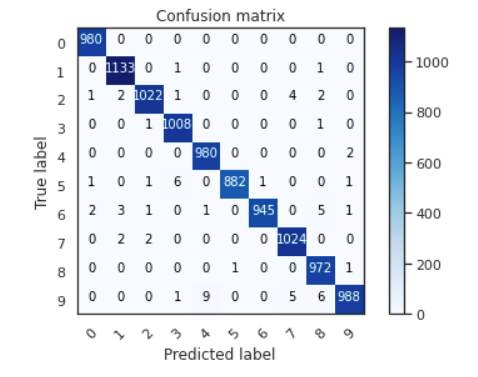
\includegraphics[width=0.8\linewidth]{img/vgg5}
	\caption{}
	\label{fig:vgg5}
\end{figure}

Además, la precisión obtenida es: \mint{python}{Test Accuracy:  0.9933999}

Podemos observar que la precisión ha aumentado con respecto a la que obtuvimos con LeNet, lo cual era de esperar pues esta arquitectura es extremadamente sencilla y no podemos esperar resultados espectaculares con la misma, al contratio que VGGNet, que es bastante más compleja y más profunda, por lo que los resultados esperables son mejores. 

En cambio, si nos fijamos en los resultados obtenidos con las otras dos estructuras de redes convolucionales que probamos, también sencillas, nos damos cuenta de que VGGNet ha empeorado estos resultados. Esto puede ser debido a que hemos partido de dicha red pre-entrenada sobre un conjunto de datos que no tiene las mismas características que nuestro problema, no se parecen lo suficiente como para poder usar la red pre-entrenada casi en su totalidad. Además, al ser una red mucho más compleja, es más difícil de entrenar, de manera que es necesario una configuración más exahustiva de sus parámetros. Quizás con otros parámetros hubiera ofrecido mejores resultados. Vemos, por lo tanto, que una red más sencilla es suficiente para resolver este problema y es más fácil de entrenar. 

\subsubsection{Con Data Augmentation}
Podemos repetir todo el procedimiento anterior pero entrenando las últimas capas que introdujimos nuevas y realizando el fine-tuning sobre el conjunto de entrenamiento aumentado usando \mintinline{python}{ImageDataGenerator}, como hicimos para las redes de doble y triple capa convolucional del apartado 3.2. 

Con el modelo entrenado sobre este nuevo conjunto de datos, la matriz de confusión obtenida para el conjunto de test ha sido:
\begin{figure}[H]
	\centering
	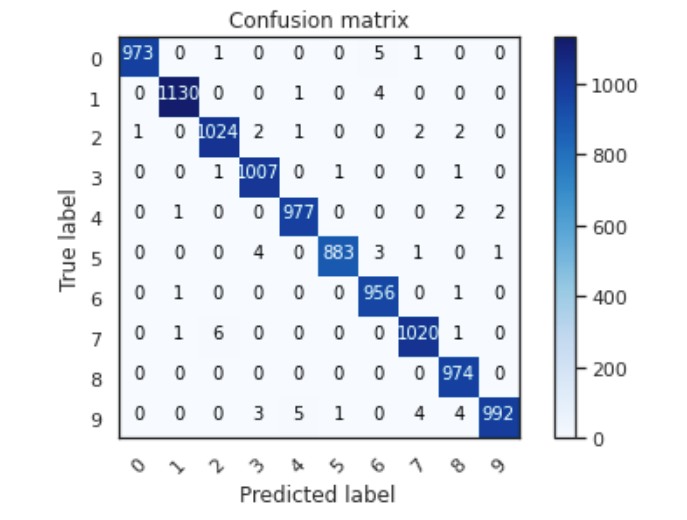
\includegraphics[width=0.8\linewidth]{img/vgg6}
	\caption{}
	\label{fig:vgg6}
\end{figure}

y la precisión: \mint{python}{Test Accuracy:  0.9936}

El valor de la precisión ha aumentado ligeramente con respecto a la precisión obtenida para el modelo entrenado sobre el conjunto de datos sin aumento, puesto que ahora se dispone de más datos para el entrenamiento. Sin embargo, sigue sin ser mejor que el valor obtenido para las redes que estudiamos en el punto 3.2, por los motivos ya comentados. 
\newpage
\subsection{Tabla comparativa de resultados}

Resumimos en la siguiente tabla los valores de precisión obtenidos para los diferentes modelos que hemos analizado:
\begin{table}[H]
	\caption{}
	\begin{tabular}{|l|c|c|}
		\hline
		\multicolumn{1}{|c|}{\textbf{}} & \textbf{Con Data Augmentation} & \textbf{Sin Data Augmentation} \\ \hline
		\textbf{LeNet} & -- & 0.9897 \\ \hline
		\textbf{Doble capa convolucional} & 0.99599 & -- \\ \hline
		\textbf{Triple capa convolucional} & 0.99739 & -- \\ \hline
		\textbf{VGG16} & 0.9936 & 0.99339 \\ \hline
	\end{tabular}
	\label{}
\end{table}

Los posibles motivos por los que se presentan estas diferencias entre la precisión de los distintos modelos ya se han ido comentando en los apartados anteriores. 
  
\section{Planteamiento de futuro}
Si pudiera trabajar durante seis meses en este problema, haría lo siguiente:
\begin{enumerate}
	\item En primer lugar, intentaría estudiar y entender los distintos tipos de arquitecturas de redes convolucionales que existen y en las que no he tenido tiempo de profundizar, pero que me habría gustado llegar a entender y probar.  Algunas de estas arquitecturas son las siguientes:
	\begin{itemize}
		\item \textbf{ResNet} (Residual Neural Networks), basadas en el concepto de bloque residual, a la salida de una capa se le suma la entrada de la misma y se usa el resultado como entrada para la siguiente capa. Permiten obtener redes convolucionales muy profundas con un buen rendimiento y un coste computacional asequible.
		\item \textbf{Inception}, cuya idea es usar filtros de distintos tamaños al mismo nivel, obteniéndose redes más anchas en lugar de más profundas. 
		\item \textbf{DenseNet} (Dense Neural Networks), usan la misma idea que ResNet, donde cada capa pasa sus mapas de características salientes como entrada a cada una de las capas siguientes.
		\item \textbf{CapsNet} (Capsule Networks), que usan vectores en lugar de escalares para realizar las operaciones de cada nodo de la red. Estos vectores contienen información espacial como el tamaño o la orientación, de forma que se tiene en cuenta mucha más información de las imágenes. Este tipo de redes ofrecen los mejores resultados para el problema de MNIST. 
		\item AlexNet, Xception Net, ....
	\end{itemize}
	Aplicaría cada una de estas arquitecturas por separado a nuestro problema, partiendo de ellas pre-entrenadas por supuesto, y analizaría cual ofrece los mejores resultados
	\item Una vez que haya probado los distintos modelos y tenga claro cuales son los mejores para nuestro problema, intentaría realizar un \textbf{Stacking} de ellos, probando distintas combinaciones, aplicándolos a nuestro problema y analizando los resultados.
	\item Otra opción a considerar sería usar para llevar a cabo la clasificación, al final de todas las capas convolucionales y una vez extraídas las características de las imágenes, distintos tipos de clasificadores, como Random Forest, SVM o Knn (con sus parámetros adecuadamente configurados), en lugar de redes neuronales. Incluso se podría tomar como clasificador un Stacking de distintos modelos, incluyendo las redes neuronales. Analizaría los resultados obtenidos con cada uno de los clasificadores por separado y los obtenidos considerando un Stacking de los que ofrecieran los mejores resultados. 
\end{enumerate}

Después de probar todo esto, decidiría cuál de todas las opciones y combinaciones de clasificadores y arquitecturas es la mejor para resolver este problema y, si consiguiera resultados novedosos, a lo mejor hasta publicaría un Paper, quién sabe $ :D $


Si me sobrara tiempo, también podría considerar una modificación de este problema para hacerlo más interesante. En lugar de partir de todo el conjunto de imágenes de entrenamiento, se puede partir de sólo algunas de ellas, digamos 1000 imágenes. Entrenaría entonces sobre este nuevo cojunto (con data augmentation como hemos visto en el código probado en la parte de estudio experimental) el mejor de los modelos obtenidos con el conjunto original y vería los resultados sobre el conjunto de test. Este modelo, sin embargo, no tiene por qué ser el mejor para el nuevo problema (como tenemos pocos datos puede producirse sobreajuste, entre otras cosas), por lo que debería probar de nuevo todos los modelos anteriores y repetir el procedimiento llevado a cabo antes. Aunque en primer lugar estudiaría cómo tratar con este tipo de problemas, en los que el conjunto de datos de entrenamiento es muy pequeño, pues hay distintas técnicas para estos casos. 


\newpage
\begin{thebibliography}{9}
\bibitem{1} 	
\url{https://www.kaggle.com/c/digit-recognizer/discussion/61480}

\bibitem{2} 
\url{https://www.youtube.com/watch?v=iaSUYvmCekI}

\bibitem{3} 
\url{https://www.youtube.com/watch?v=JB8T_zN7ZC0}

\bibitem{4} 
\url{https://medium.com/coinmonks/an-introduction-to-cnns-and-a-step-by-step-model-of-a-digit-recognizer-using-mnist-database-in-f4ea6af06d77}

\bibitem{5} 
\url{https://www.geeksforgeeks.org/cnn-introduction-to-pooling-layer/}
\bibitem{6} 
\url{https://keras.io/api/layers/activations/}
\bibitem{7} 
\url{http://vision.stanford.edu/cs598_spring07/papers/Lecun98.pdf}
\bibitem{8} 
\url{https://towardsdatascience.com/understanding-and-implementing-lenet-5-cnn-architecture-deep-learning-a2d531ebc342}
\bibitem{9} 
\url{https://medium.com/towards-artificial-intelligence/the-architecture-implementation-of-lenet-5-eef03a68d1f7}
\bibitem{10} 
\url{https://github.com/RichmondAlake/tensorflow_2_tutorials/blob/master/13_lenet-5.ipynb}
\bibitem{11} 
\url{http://yann.lecun.com/exdb/mnist/}
\bibitem{12} 
\url{https://stackoverflow.com/questions/40427435/extract-images-from-idx3-ubyte-file-or-gzip-via-python}
\bibitem{13}
\url{https://www.kaggle.com/c/digit-recognizer/overview}
\bibitem{14}
\url{https://www.kaggle.com/sauravjoshi23/digit-recognition-using-cnn-99-835-acc-top-4}
\bibitem{15}
\url{https://adeshpande3.github.io/A-Beginner%27s-Guide-To-Understanding-Convolutional-Neural-Networks-Part-2/}
\bibitem{16}
\url{https://www.tensorflow.org/api_docs/python/tf/keras/preprocessing/image/ImageDataGenerator}
\bibitem{17}
\url{https://medium.com/analytics-vidhya/vggnet-architecture-explained-e5c7318aa5b6}
\bibitem{18}
\url{https://towardsdatascience.com/architecture-comparison-of-alexnet-vggnet-resnet-inception-densenet-beb8b116866d}
\bibitem{19}
\url{https://www.youtube.com/watch?v=_2EHcpg52uU&feature=youtu.be}
\bibitem{20}
\url{https://towardsdatascience.com/step-by-step-guide-to-using-pretrained-models-in-keras-c9097b647b29}
\bibitem{21}
\url{https://towardsdatascience.com/a-simple-and-intuitive-explanation-of-hintons-capsule-networks-b59792ad46b1}
\bibitem{22}
\url{https://www.sciencedirect.com/science/article/abs/pii/S1566253520302542}
\bibitem{23}
\url{https://keras.io/api/applications/vgg/#vgg16-function}

\end{thebibliography}
\end{document}
